\chapter{\IfLanguageName{dutch}{Stand van zaken}{State of the art}}%
\label{ch:stand-van-zaken}

% Tip: Begin elk hoofdstuk met een paragraaf inleiding die beschrijft hoe
% dit hoofdstuk past binnen het geheel van de bachelorproef. Geef in het
% bijzonder aan wat de link is met het vorige en volgende hoofdstuk.

% Pas na deze inleidende paragraaf komt de eerste sectiehoofding.


% TODO: GDPR regulations about storing face data/imgs

\section{Authentication in Digital Security}
Authentication is the process of verifying the identity of users attempting to access digital systems or online services. 
Commonly used methods include knowledge-based authentication (passwords), possession-based methods (tokens), and 
biometric methods like fingerprints and facial recognition \autocite{Pant2022}. Passwords remain dominant due to 
their simplicity and widespread acceptance, but face security issues including password reuse, phishing, and 
brute-force attacks \autocite{Ophoff2021}. For users with cognitive or motor disabilities, these issues are 
further complicated by difficulties in recalling or accurately inputting passwords \autocite{Rochford2014}.

\section{Accessibility Challenges in Authentication}
Individuals with cognitive disabilities, such as memory disorders or conditions like dyslexia, often struggle with remembering complex passwords, resulting in frequent authentication failures and frustration \autocite{Farid2019, Ophoff2021}. Those with motor disabilities, including conditions like Parkinson's disease or cerebral palsy, face physical challenges in typing passwords accurately \autocite{Renaud2020}. The Web Content Accessibility Guidelines (WCAG) highlight the importance of designing authentication systems that minimize these cognitive and physical burdens \autocite{Brewer2023}.

\vspace{4\baselineskip}
\section{Facial Recognition Technology}
Facial recognition works by identifying and verifying individuals from digital images or videos using various algorithmic approaches, including traditional image processing methods and modern deep learning techniques. Notable algorithms include Haar cascades, Eigenfaces, Local Binary Patterns Histograms (LBPH), and Convolutional Neural Networks (CNNs) \autocite{ElSayed2015}. The evolution of deep learning, particularly CNN-based approaches, has significantly enhanced accuracy and reliability, making facial recognition robust even under challenging conditions like variations in lighting, angle, or facial expressions \autocite{Zhang2020}.

\section{Face Recognition as a Biometric Solution}
Biometric authentication, particularly facial recognition, is gaining popularity as it significantly reduces the cognitive and physical effort required by traditional password-based methods \autocite{Furnell2022}. 
Unlike passwords, biometric data are unique physical attributes of an individual, providing an inherent security advantage by eliminating risks associated with knowledge-based authentication methods, 
such as forgetting or sharing passwords \autocite{Pant2022}.

Facial recognition stands out as particularly promising because it is intuitive, does not require manual dexterity, and can be seamlessly integrated into daily digital interactions \autocite{Bhatt2011}. However, biometric systems are not without limitations. Spoofing attacks, privacy concerns, and the requirement for consistent lighting and camera quality present technical and ethical considerations that must be carefully managed \autocite{Kuznetsov2024, Bahia2024}.


\subsection{Comparison of Facial Recognition Libraries}

\subsubsection{OpenCV (Java)}
OpenCV is a widely used open-source library offering classical computer vision techniques such as Haar cascades and LBPH. While effective in controlled environments, it typically requires server-side or desktop-based implementations, limiting its applicability for client-side web applications \autocite{Dominguez2017}.

\subsubsection{face\_recognition in Python}  
The face\_recognition library, built on dlib, is renowned for its accuracy and pre-trained deep learning models. \textcite{Zhang2020} highlight that it excels in applications requiring precision, utilizing techniques like CNN-based face encodings for high-quality results. However, its reliance on Python and backend processing makes it less suitable for client-side, browser-based implementations like those required in this project.

\subsubsection{face-api.js (JavaScript)}
face-api.js, built on TensorFlow.js, runs entirely in the browser, providing a privacy-centric, client-side solution suitable for real-time applications \autocite{Vageele2024}. Its key benefits include privacy (no server-side data transfer), compatibility with modern web frameworks, and modularity for lightweight and efficient real-time processing. These features align closely with the project's emphasis on usability, accessibility, and security, making face-api.js the optimal choice for this research.

\section{Security Considerations for Biometric Authentication}
While facial recognition enhances accessibility, it also introduces specific security concerns. Common vulnerabilities include spoofing attacks using photos or video recordings and data privacy issues related to biometric data storage \autocite{Bowyer2006, Bahia2024}. Modern mitigation strategies include:
\begin{itemize}
\item \textbf{Liveness Detection:} Techniques to ensure the presence of a real, live user rather than a static image or video \autocite{Kuznetsov2024}.
\item \textbf{Local Data Processing:} Client-side processing prevents the transmission of sensitive biometric data, enhancing privacy.
\item \textbf{Multi-factor Authentication (MFA):} Combining biometric data with other authentication methods to provide layers of security and protect against vulnerabilities inherent in single-method authentication systems \autocite{Furnell2022}.
\end{itemize}

\section{Current Limitations in Password Managers}
Password managers simplify password management by securely storing and auto-filling credentials but commonly rely on a master password, perpetuating cognitive and motor accessibility issues. This approach is problematic for users who struggle with memory recall or precise typing \autocite{IALabs2024}. While MFA offers increased security, it often introduces additional complexity that further burdens users with disabilities. Current systems have limited inclusivity and accessibility, reinforcing the need for more intuitive solutions.

\section{Database Options for Client\textendash Side Password Storage}
\label{sec:db-options}

A password manager must choose a local datastore that balances footprint,
offline capability, security, and future synchronisation needs.  The five
candidates below are summarised with literature references and official
documentation links; each paragraph is kept within seven lines for brevity.

\subsection*{SQLite}
\textcite{Gaffney2022} show that SQLite embeds the entire ACID-compliant
engine in a single file of only a few-hundred-kB, requiring no server
process.  Its dynamic typing allows flexible schemas \autocite{Corovcak2025}.
Because it lacks native user authentication, security depends on OS file
permissions or extensions such as SQLCipher \autocite{Corovcak2025}.
Official documentation confirms the zero-config model and SQL feature set
\autocite{sqlLiteDoc2025}.  These traits make SQLite ideal for an offline,
single-device password vault, provided the file is encrypted at rest.

\subsection*{PostgreSQL}
PostgreSQL's client-server design provides robust concurrency and rich SQL
features after 35-years of development \autocite{Gkamas2022}.  It supports
role-based access control and TLS for data in transit, yet the community
edition offers no built-in at-rest encryption—administrators must use
\textit{pgcrypto} or file-system measures \autocite{Crunchy2024,
PostgreSQL2025}.  A local instance typically consumes hundreds of-MB of RAM,
which is heavy for a mobile vault.  Hence PostgreSQL is secure and scalable,
but over-provisioned for a single-user client.

\subsection*{MongoDB}
MongoDB stores JSON-like documents in flexible collections and scales
horizontally \autocite{Miryala2024}.  A \texttt{mongod} process needs 1-2-GB
RAM even for modest use \autocite{Dahunsi2021}.  Community builds provide
authentication and TLS, yet encryption at rest is Enterprise-only
\autocite{PrismaMongoEnc, MongoDB2025}, so disk encryption or field-level
crypto is required.  Misconfiguration has repeatedly exposed databases,
underscoring the need for hardened defaults \autocite{SqlLite2025}.  The
server footprint makes MongoDB ill-suited to a purely offline desktop
password manager.

\subsection*{Couchbase Lite}
Couchbase Lite embeds a document store inside the app and syncs through
Sync Gateway when online \autocite{Pal2016}.  Its metadata inflates on-disk
size versus SQLite, yet runtime demands remain mobile-friendly
\autocite{Gkamas2022}.  The Enterprise build supports 256-bit AES encryption
of the local DB \autocite{CouchbaseEncryption, CouchbaseDoc2025}.  Because it
executes in the app's sandbox, further authentication is handled by the host
application.  These qualities make Couchbase Lite attractive for an
offline-first vault that may later sync across devices.

\subsection*{Firebase Cloud Firestore}
Firestore is a serverless NoSQL service that caches data locally and
synchronises transparently once connectivity returns \autocite{FirebaseDoc2025}.
Security combines Firebase Authentication with declarative Firestore Rules,
while Google encrypts data in transit and at rest \autocite{FirebaseSecurity2025}.
This offloads database maintenance but requires Internet access for initial
login and long-term storage.  Firestore therefore suits a multi-device,
cloud-centric password manager but cedes full data custody to Google.


\section{Cryptographic Security in Password Managers}
Secure storage of credentials is fundamental in password management.  
In this project, every cryptographic operation executes client-side with the
\texttt{crypto-js} library \autocite{CryptoJS2024}, combining AES-256 for
confidentiality and PBKDF2 for key derivation.  AES supplies a
NIST-approved block cipher \autocite{NISTFIPS197}, while PBKDF2's 10\,000
iterations and per-installation salt greatly raise the cost of brute-force
attacks \autocite{RFC8018}.  Keeping both encryption and decryption in the
browser ensures plaintext credentials or biometric images never leave the
device, aligning with OWASP key-management guidance
\textcite{OWASPKeyMgmt2025}.

\subsubsection{Crypto-js}  
The \texttt{crypto-js} library offers JavaScript implementations of AES,
PBKDF2, and other standard algorithms through a concise API optimised for the
browser.  Its widespread adoption and open-source governance mean the code
base is continuously scrutinised and updated for vulnerabilities
\autocite{CryptoJS2024}.

\subsubsection{AES}  
AES-256 encrypts both passwords and face images, providing a large key space
and proven resistance to cryptanalysis.  Defined in FIPS 197, AES remains the
de-facto standard for protecting electronic data across government and
industry \autocite{NISTFIPS197}. 

\subsubsection{Encryption Key Handling}  
Each encryption key is derived in the browser at login and kept only in
memory; it is never persisted or sent to the backend.  This client-centric
approach follows OWASP key-management recommendations, ensuring a server
breach alone cannot expose decryption keys
\autocite{OWASPKeyMgmt2025}. 

\subsubsection{PBKDF2}  
PBKDF2, specified in RFC 8018, transforms the user's secret into a strong
256-bit key using 10\,000 iterations and a unique 16-byte salt.  Iterative
key stretching slows dictionary attacks, while the salt thwarts rainbow
tables \autocite{RFC8018}.

\section{Usability and Accessibility Standards}
Accessibility in digital solutions adheres to guidelines such as WCAG, which outline best practices for minimizing cognitive load, ensuring interface clarity, and reducing physical input requirements. Adopting these standards ensures the password manager prototype remains usable for individuals with various disabilities \autocite{Brewer2023}. Inclusive design principles further emphasize the need to involve users with disabilities in the development process to validate and refine usability \autocite{Lazar2015}.

\subsection{WCAG 2.1 Compliance Framework}
A comprehensive approach to accessibility requires systematic mapping of features against established standards. The table below provides a traceability matrix that maps the password manager's features to the Web Content Accessibility Guidelines (WCAG 2.1) success criteria. This matrix serves as both a design reference and a verification tool to ensure all accessibility requirements are addressed in the implementation phase. When we discuss the usability study design in Chapter~\ref{ch:methodologie}, we will reference this matrix to highlight which criteria were empirically verified through user testing.

\begin{table}[htbp]
  \centering
  \small
  \begin{tabular}{|p{2.5cm}|p{1.5cm}|p{4cm}|p{4cm}|p{1.2cm}|}
    \hline
    \textbf{WCAG 2.1} & \textbf{Con-} & \textbf{Features} & \textbf{Evidence / Implementation} & \textbf{Status} \\
    \textbf{Success} & \textbf{formance} & & & \\
    \textbf{Criterion} & \textbf{Level} & & & \\ \hline
    
    1.1.1 Non-text Content & A & Face-registration and authentication UI, credential icons, action buttons & alt text for static images; ARIA labels (e.g. aria-label="Capture selfie") on camera controls & Pass \\ \hline
    
    1.3.1 Info \& Relationships & A & Modal forms for Add / Edit Credential, list view of saved credentials & Implemented with semantic HTML elements (\texttt{<form>}, \texttt{<label>}, \texttt{<ul>/<li>}); programmatic labels bound to inputs & Pass \\ \hline
    
    1.3.2 Meaningful Sequence & A & React component hierarchy for registration \& login flows & DOM order matches visual order; logical tab order verified with keyboard & Pass \\ \hline
    
    1.3.4 Orientation & AA & Responsive layout (CSS Flex/Grid) & UI adapts to both portrait and landscape on mobile; no fixed-orientation lock & Pass \\ \hline
    
    1.4.3 Contrast (Minimum) & AA & Global Tailwind theme & Colour palette tested with WCAG contrast checker: all text/background combinations $\geq$ 4.5:1 & Pass \\ \hline
    
    1.4.5 Images of Text & AA & Credential list, buttons & No UI element relies on rasterised text; all labels are true text & Pass \\ \hline
    
    1.4.10 Reflow & AA & Responsive UI on small screens & Tested to 320 px width without horizontal scroll & Pass \\ \hline
    
    1.4.11 Non-text Contrast & AA & Icon buttons, focus rings & SVG icons meet 3:1 contrast; focus outline uses high-contrast colour & Pass \\ \hline
    
    2.1.1 Keyboard & A & All interactive controls & tabIndex flows through modals and lists; face-capture can be triggered with Enter key & Pass \\ \hline
    
    2.1.2 No Keyboard Trap & A & Modal dialogs & Esc, Tab and Shift+Tab correctly move focus or close modal & Pass \\ \hline
  \end{tabular}
  \caption[WCAG 2.1 Traceability Matrix]{WCAG 2.1 Traceability Matrix for the Face-Based Password Manager. This matrix maps features of the prototype to relevant Web Content Accessibility Guidelines success criteria, demonstrating how the design addresses accessibility requirements.}
  \label{tab:wcag-matrix}
\end{table}

\begin{table}[htbp]
  \centering
  \small
  \begin{tabular}{|p{2.5cm}|p{1.5cm}|p{4cm}|p{4cm}|p{1.2cm}|}
    \hline
    \textbf{WCAG 2.1} & \textbf{Con-} & \textbf{Features} & \textbf{Evidence / Implementation} & \textbf{Status} \\
    \textbf{Success} & \textbf{formance} & & & \\
    \textbf{Criterion} & \textbf{Level} & & & \\ \hline
    
    2.2.1 Timing Adjustable & A & Face-capture countdown & 5-second default, user can extend to 15 s via settings & Pass \\ \hline
    
    2.3.1 Three Flashes or Below & A & Toast animations & All animations < 3 flashes/sec; none are bright flashes & Pass \\ \hline
    
    2.4.3 Focus Order & A & Credential list, modals & Logical sequential focus verified with screen-reader & Pass \\ \hline
    
    2.4.4 Link Purpose & A & External links in footer/help & Link text describes destination (e.g. "WCAG Quick-Ref") & Pass \\ \hline
    
    2.4.7 Focus Visible & AA & Custom focus outline & Uses 2 px outline + 4 px offset to meet visibility & Pass \\ \hline
    
    3.2.1 On Focus & A & Input fields, buttons & No unexpected context changes on focus & Pass \\ \hline
    
    3.2.2 On Input & A & Credential forms & Only explicit Save triggers state change; live form validation announced politely & Pass \\ \hline
    
    3.3.1 Error Identification & A & Form validation & Error messages displayed inline and exposed via aria-describedby & Pass \\ \hline
    
    3.3.2 Labels or Instructions & A & All form inputs, face-capture & Clear labels ("Email Address") and helper text ("Look straight at the camera") & Pass \\ \hline
    
    4.1.1 Parsing & A & React front-end templates & JSX compiles to valid HTML; no duplicate IDs & Pass \\ \hline
    
    4.1.2 Name, Role, Value & A & Custom components (Modal, Button, Toast) & Roles and states exposed with ARIA (role="dialog", aria-modal="true", aria-live="polite") & Pass \\ \hline
  \end{tabular}
  \caption[WCAG 2.1 Traceability Matrix (continued)]{WCAG 2.1 Traceability Matrix for the Face-Based Password Manager (continued).}
  \label{tab:wcag-matrix-cont}
\end{table}


% \begin{figure}
%   \centering
%   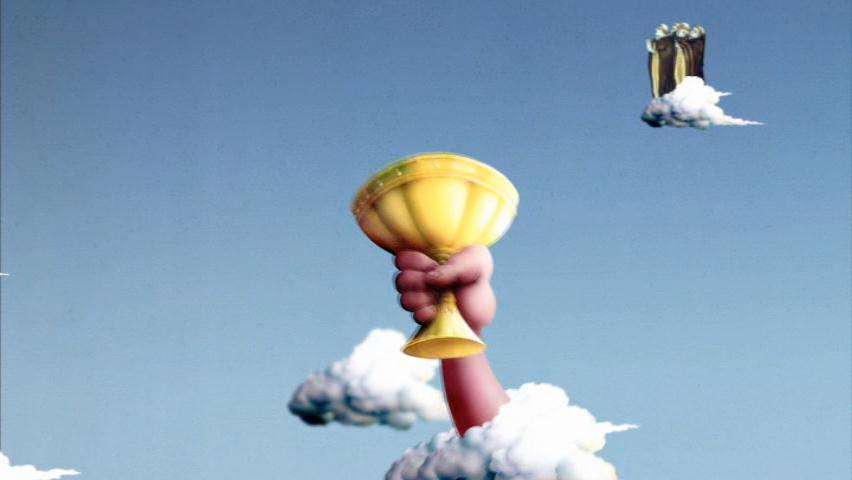
\includegraphics[width=0.8\textwidth]{grail.jpg}
%   \caption[Voorbeeld figuur.]{\label{fig:grail}Voorbeeld van invoegen van een figuur. Zorg altijd voor een uitgebreid bijschrift dat de figuur volledig beschrijft zonder in de tekst te moeten gaan zoeken. Vergeet ook je bronvermelding niet!}
% \end{figure}

% \begin{listing}
%   \begin{minted}{python}
%     import pandas as pd
%     import seaborn as sns

%     penguins = sns.load_dataset('penguins')
%     sns.relplot(data=penguins, x="flipper_length_mm", y="bill_length_mm", hue="species")
%   \end{minted}
%   \caption[Voorbeeld codefragment]{Voorbeeld van het invoegen van een codefragment.}
% \end{listing}

% \lipsum[7-20]

% \begin{table}
%   \centering
%   \begin{tabular}{lcr}
%     \toprule
%     \textbf{Kolom 1} & \textbf{Kolom 2} & \textbf{Kolom 3} \\
%     $\alpha$         & $\beta$          & $\gamma$         \\
%     \midrule
%     A                & 10.230           & a                \\
%     B                & 45.678           & b                \\
%     C                & 99.987           & c                \\
%     \bottomrule
%   \end{tabular}
%   \caption[Voorbeeld tabel]{\label{tab:example}Voorbeeld van een tabel.}
% \end{table}
